\documentclass[multi=tikzpicture,border=10pt]{standalone}
\usepackage{fontspec}
\usepackage{amssymb}
\usepackage{xcolor}
\usepackage{tikz}
\usetikzlibrary{arrows.meta,calc,positioning,shadows.blur}

\setmainfont{Latin Modern Sans}

\definecolor{substrate}{HTML}{1F4E79}
\definecolor{matter}{HTML}{2E7D32}
\definecolor{gauge}{HTML}{00838F}
\definecolor{cosmo}{HTML}{EF6C00}
\definecolor{dark}{HTML}{6A1B9A}
\definecolor{gravity}{HTML}{B71C1C}
\definecolor{relativity}{HTML}{AD1457}
\definecolor{method}{HTML}{616161}
\definecolor{derivedfill}{HTML}{E8F2FF}
\definecolor{condfill}{HTML}{FFF4D8}
\definecolor{openfill}{HTML}{F4E8FB}
\definecolor{importfill}{HTML}{EEEEEE}
\definecolor{retiredfill}{HTML}{FBE9E7}

\tikzset{
  root/.style={
    rounded corners=4pt,
    draw=black!58,
    line width=0.7pt,
    fill=white,
    blur shadow={shadow blur steps=4, shadow xshift=0.6pt, shadow yshift=-0.6pt, shadow opacity=16},
    align=center,
    font=\footnotesize\bfseries,
    inner xsep=6pt,
    inner ysep=5pt,
    text width=3.25cm
  },
  nodebox/.style={
    rounded corners=3pt,
    draw=black!45,
    line width=0.55pt,
    fill=white,
    align=center,
    font=\footnotesize,
    inner xsep=5pt,
    inner ysep=4pt,
    text width=3.18cm
  },
  derived/.style={fill=derivedfill, draw=substrate!70},
  conditional/.style={fill=condfill, draw=cosmo!82},
  open/.style={fill=openfill, draw=dark!82, dashed},
  imported/.style={fill=importfill, draw=method!70},
  retired/.style={fill=retiredfill, draw=red!72, densely dashed},
  treeedge/.style={line width=1.0pt, draw=black!55, -{Latex[length=2.3mm]}},
  crossedge/.style={line width=0.8pt, draw=method!70, dashed, -{Latex[length=2.0mm]}},
  edgelabel/.style={font=\scriptsize, text=black!68, fill=white, inner xsep=2pt, inner ysep=1pt, align=center},
  title/.style={font=\Large\bfseries, anchor=west},
  subtitle/.style={font=\small, text=black!62, anchor=west},
  pageid/.style={font=\tiny, text=black!50, anchor=east},
  note/.style={font=\scriptsize, text=black!68, align=left},
  legend/.style={font=\scriptsize, align=left, draw=black!18, rounded corners=3pt, fill=white, inner sep=5pt}
}

\newcommand{\treepage}[3]{%
  \path[use as bounding box] (0,0) rectangle (24,14);
  \fill[white] (0,0) rectangle (24,14);
  \node[title] at (0.45,13.45) {#1};
  \node[subtitle] at (0.45,13.02) {#2};
  \node[pageid] at (23.55,0.35) {#3};
}

\newcommand{\statuslegend}{%
  \node[legend, anchor=south west] at (0.45,0.45) {
    \textbf{Status:}
    \tikz{\node[nodebox, derived, minimum width=0.36cm, text width=0.16cm, inner sep=1pt]{};} derived/script-backed
    \quad
    \tikz{\node[nodebox, conditional, minimum width=0.36cm, text width=0.16cm, inner sep=1pt]{};} conditional
    \quad
    \tikz{\node[nodebox, open, minimum width=0.36cm, text width=0.16cm, inner sep=1pt]{};} open
    \quad
    \tikz{\node[nodebox, retired, minimum width=0.36cm, text width=0.16cm, inner sep=1pt]{};} retired
    \quad dashed arrows = non-tree dependencies
  };
}

\begin{document}

% ---------------------------------------------------------------------------
% Page 1: overview tree.
% ---------------------------------------------------------------------------
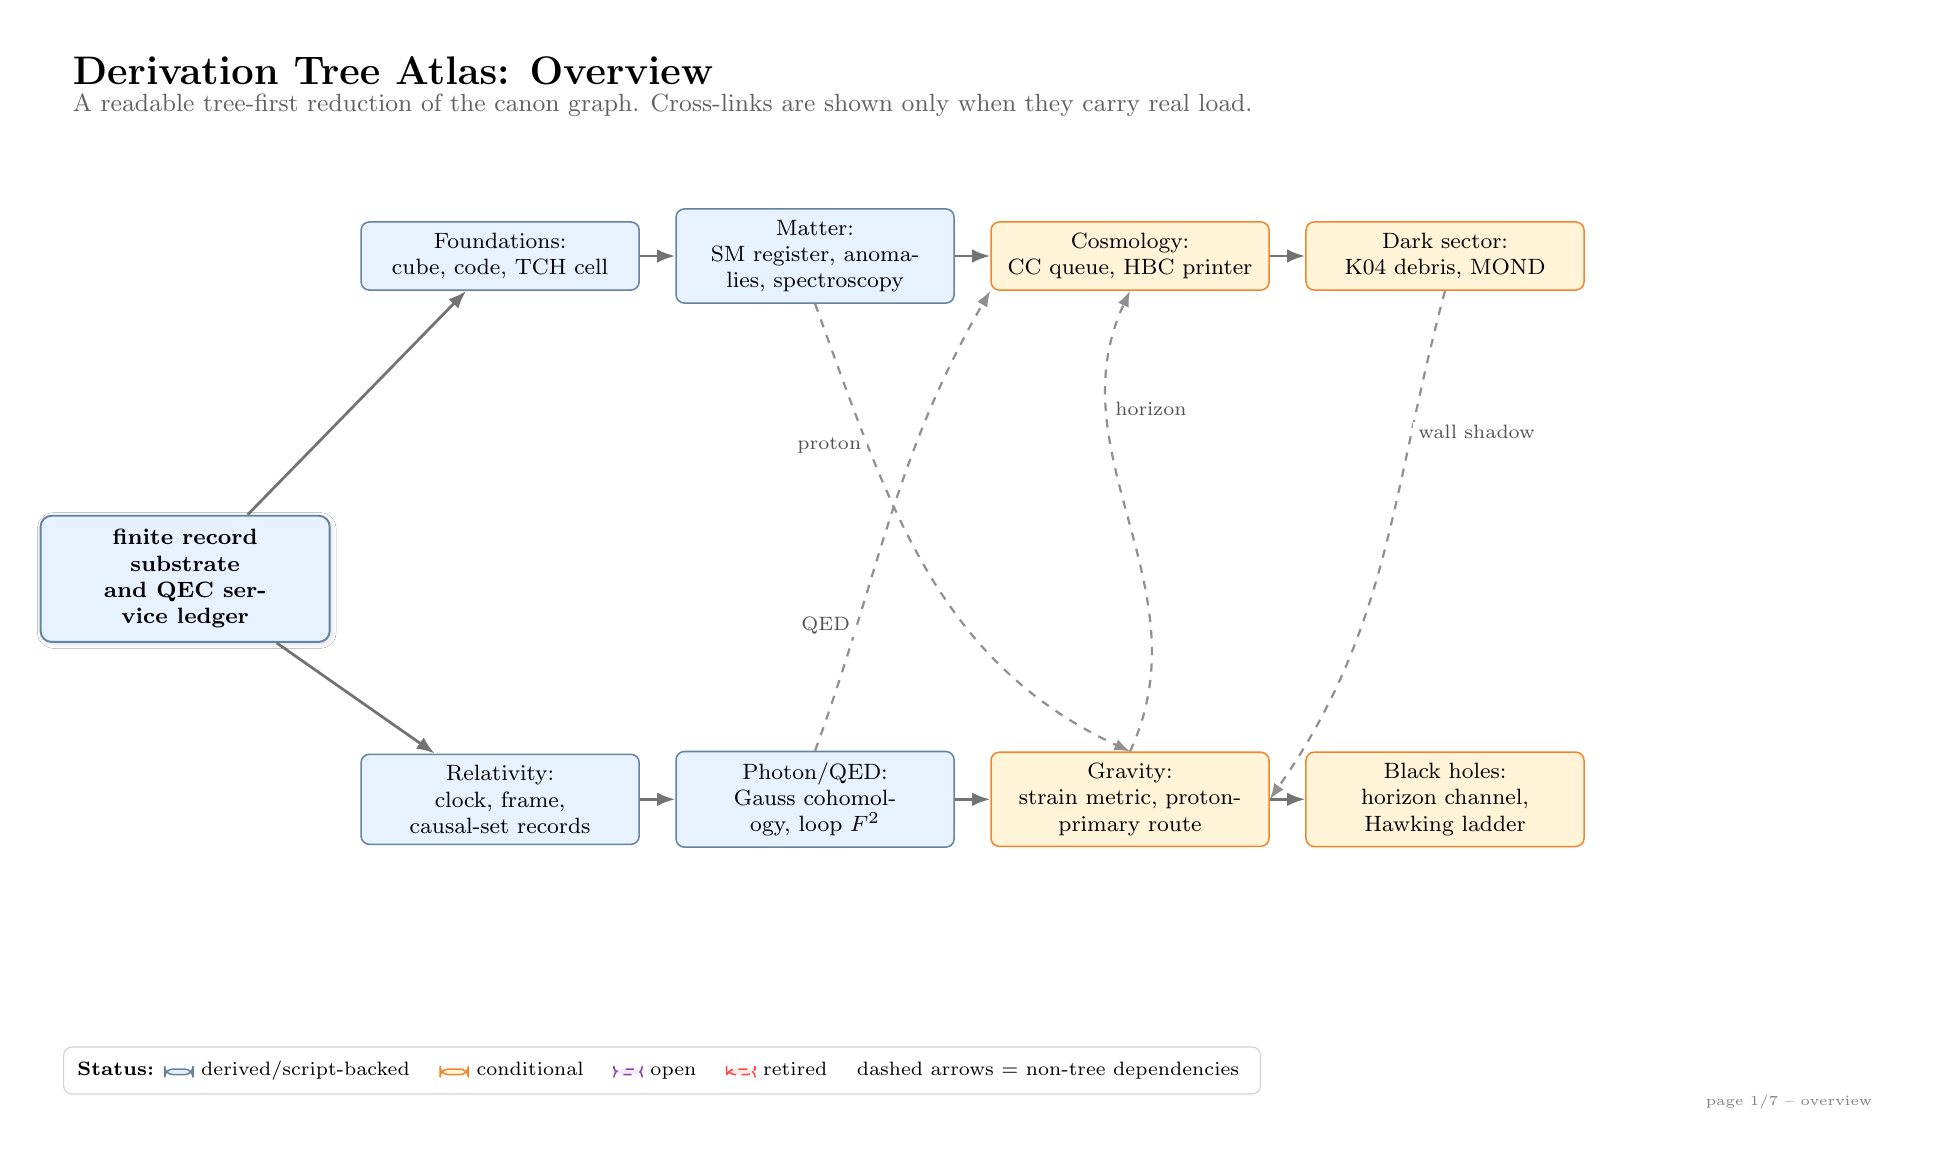
\begin{tikzpicture}[x=1cm,y=1cm]
\treepage{Derivation Tree Atlas: Overview}
  {A readable tree-first reduction of the canon graph. Cross-links are shown only when they carry real load.}
  {page 1/7 -- overview}

\node[root, derived] (spine) at (2.0,7.0) {finite record substrate\\and QEC service ledger};

\node[nodebox, derived] (found) at (6.0,11.1) {Foundations:\\cube, code, TCH cell};
\node[nodebox, derived] (matter) at (10.0,11.1) {Matter:\\SM register, anomalies, spectroscopy};
\node[nodebox, conditional] (cosmo) at (14.0,11.1) {Cosmology:\\CC queue, HBC printer};
\node[nodebox, conditional] (darkm) at (18.0,11.1) {Dark sector:\\K04 debris, MOND};

\node[nodebox, derived] (rel) at (6.0,4.2) {Relativity:\\clock, frame, causal-set records};
\node[nodebox, derived] (photon) at (10.0,4.2) {Photon/QED:\\Gauss cohomology, loop $F^2$};
\node[nodebox, conditional] (grav) at (14.0,4.2) {Gravity:\\strain metric, proton-primary route};
\node[nodebox, conditional] (bh) at (18.0,4.2) {Black holes:\\horizon channel, Hawking ladder};

\foreach \a/\b in {spine/found,found/matter,matter/cosmo,cosmo/darkm,spine/rel,rel/photon,photon/grav,grav/bh}
  \draw[treeedge] (\a) -- (\b);

\draw[crossedge] (matter.south) to[out=-70,in=155] node[edgelabel, near start, left] {proton} (grav.north);
\draw[crossedge] (grav.north) to[out=65,in=245] node[edgelabel, near end, right] {horizon} (cosmo.south);
\draw[crossedge] (darkm.south) to[out=-105,in=55] node[edgelabel, near start, right] {wall shadow} (grav.east);
\draw[crossedge] (photon.north) to[out=70,in=240] node[edgelabel, near start, left] {QED} (cosmo.south west);
\statuslegend
\end{tikzpicture}

% ---------------------------------------------------------------------------
% Page 2: foundations and methodology.
% ---------------------------------------------------------------------------
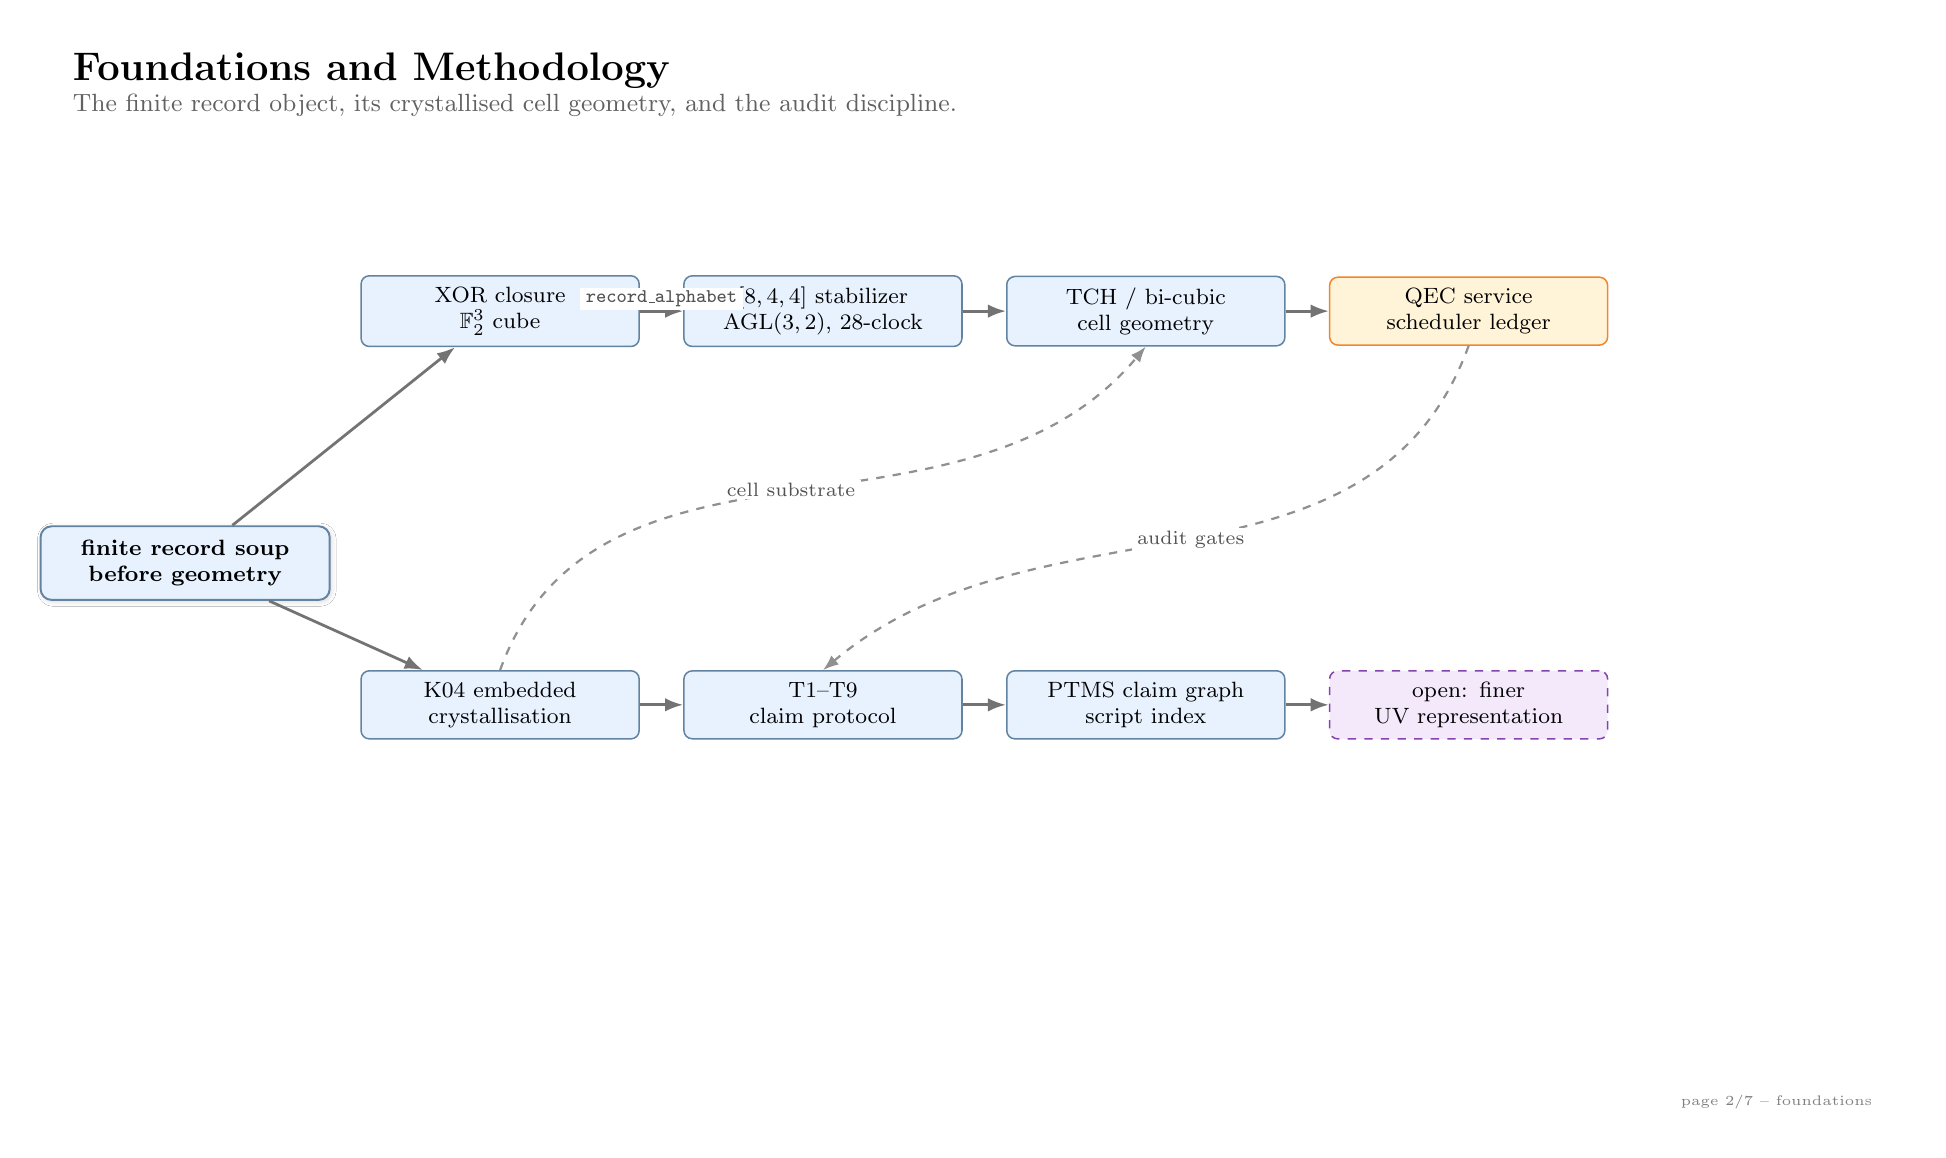
\begin{tikzpicture}[x=1cm,y=1cm]
\treepage{Foundations and Methodology}
  {The finite record object, its crystallised cell geometry, and the audit discipline.}
  {page 2/7 -- foundations}

\node[root, derived] (root) at (2.0,7.2) {finite record soup\\before geometry};

\node[nodebox, derived] (xor) at (6.0,10.4) {XOR closure\\$\mathbb F_2^3$ cube};
\node[nodebox, derived] (code) at (10.1,10.4) {$[8,4,4]$ stabilizer\\AGL$(3,2)$, 28-clock};
\node[nodebox, derived] (tch) at (14.2,10.4) {TCH / bi-cubic\\cell geometry};
\node[nodebox, conditional] (service) at (18.3,10.4) {QEC service\\scheduler ledger};

\node[nodebox, derived] (crystal) at (6.0,5.4) {K04 embedded\\crystallisation};
\node[nodebox, derived] (method) at (10.1,5.4) {T1--T9\\claim protocol};
\node[nodebox, derived] (ptms) at (14.2,5.4) {PTMS claim graph\\script index};
\node[nodebox, open] (uv) at (18.3,5.4) {open: finer\\UV representation};

\draw[treeedge] (root) -- (xor);
\draw[treeedge] (xor) -- node[edgelabel, above] {\texttt{record\_alphabet}} (code);
\draw[treeedge] (code) -- (tch);
\draw[treeedge] (tch) -- (service);
\draw[treeedge] (root) -- (crystal);
\draw[treeedge] (crystal) -- (method);
\draw[treeedge] (method) -- (ptms);
\draw[treeedge] (ptms) -- (uv);
\draw[crossedge] (service.south) to[out=-110,in=40] node[edgelabel] {audit gates} (method.north);
\draw[crossedge] (crystal.north) to[out=70,in=230] node[edgelabel] {cell substrate} (tch.south);

\end{tikzpicture}

% ---------------------------------------------------------------------------
% Page 3: matter and gauge.
% ---------------------------------------------------------------------------
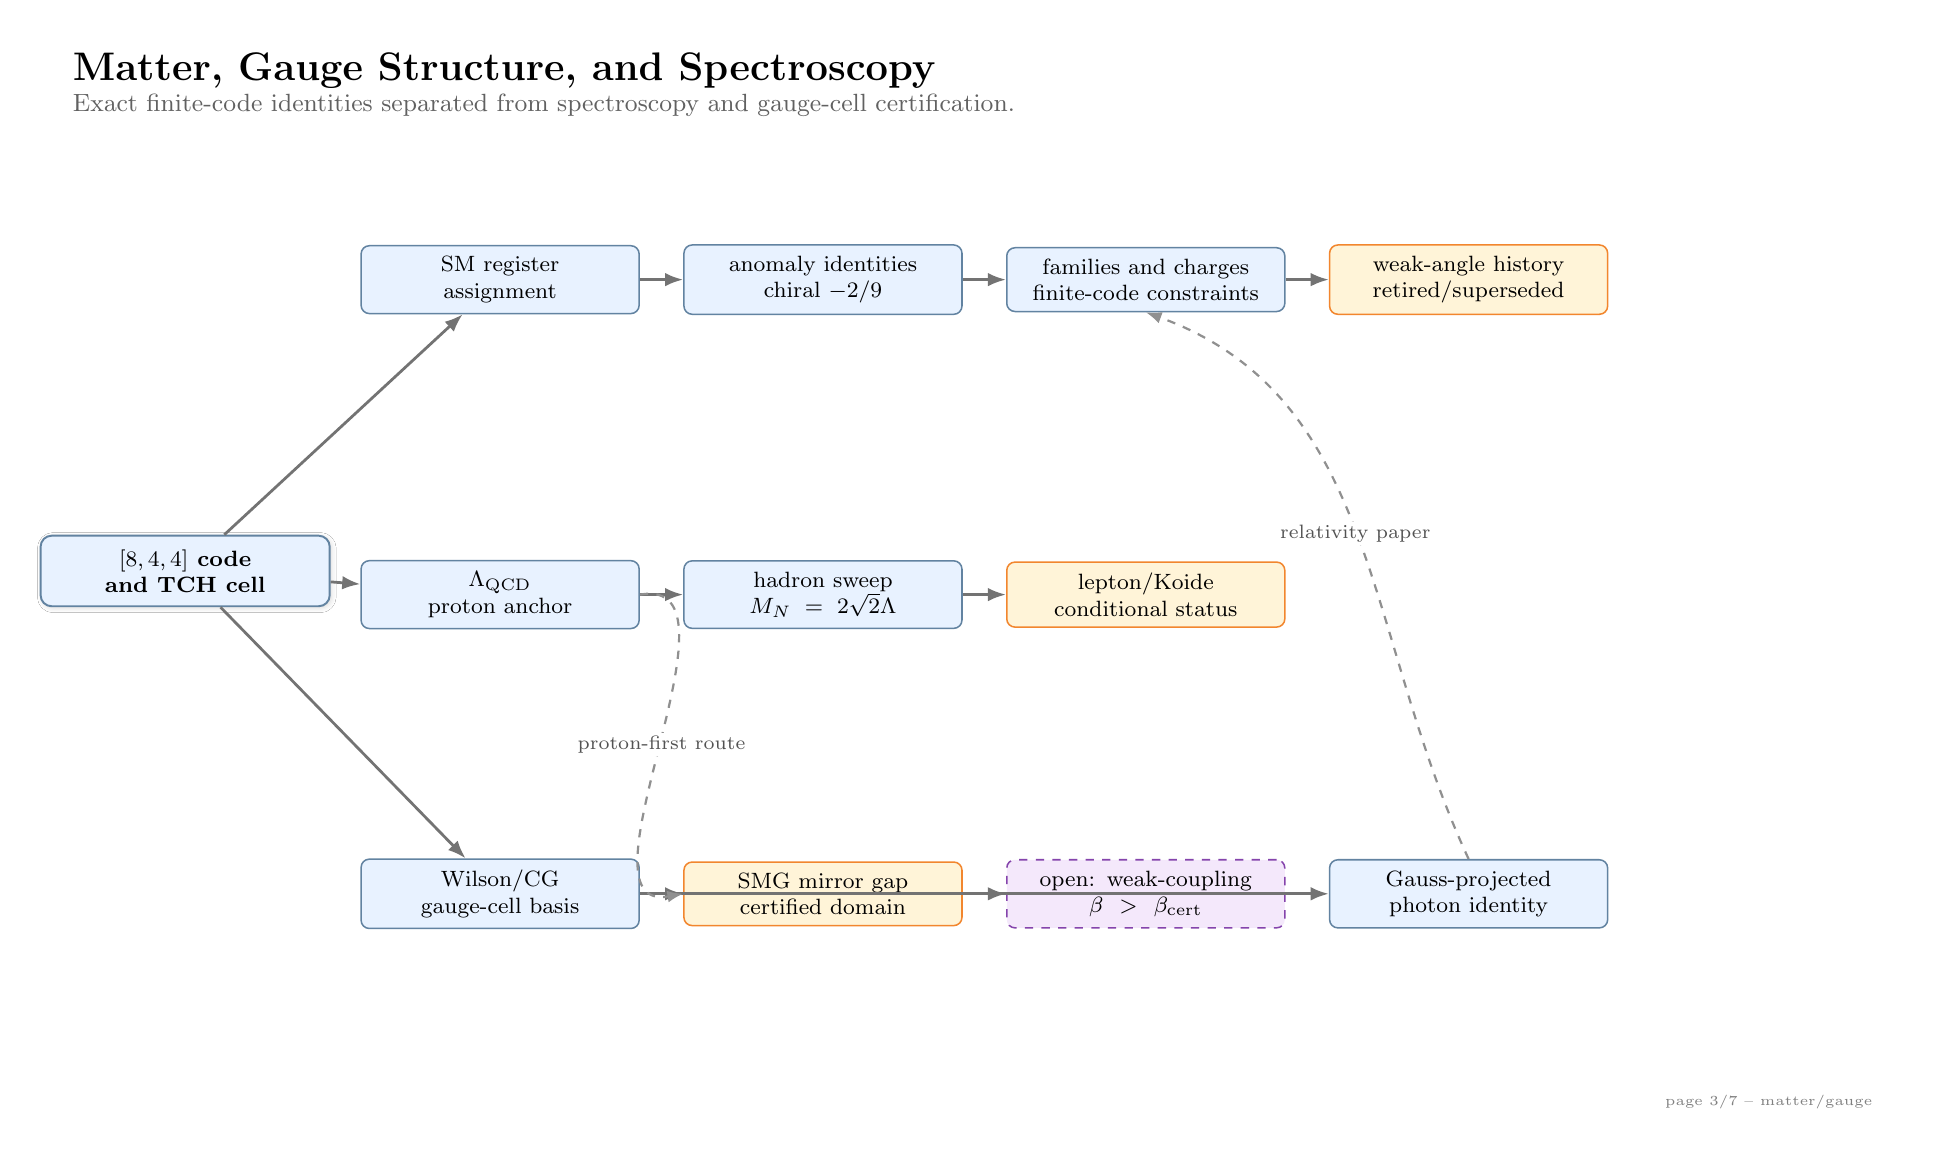
\begin{tikzpicture}[x=1cm,y=1cm]
\treepage{Matter, Gauge Structure, and Spectroscopy}
  {Exact finite-code identities separated from spectroscopy and gauge-cell certification.}
  {page 3/7 -- matter/gauge}

\node[root, derived] (root) at (2.0,7.1) {$[8,4,4]$ code\\and TCH cell};

\node[nodebox, derived] (sm) at (6.0,10.8) {SM register\\assignment};
\node[nodebox, derived] (anom) at (10.1,10.8) {anomaly identities\\chiral $-2/9$};
\node[nodebox, derived] (fam) at (14.2,10.8) {families and charges\\finite-code constraints};
\node[nodebox, conditional] (weak) at (18.3,10.8) {weak-angle history\\retired/superseded};

\node[nodebox, derived] (lambda) at (6.0,6.8) {$\Lambda_{\rm QCD}$\\proton anchor};
\node[nodebox, derived] (hadron) at (10.1,6.8) {hadron sweep\\$M_N=2\sqrt2\Lambda$};
\node[nodebox, conditional] (koide) at (14.2,6.8) {lepton/Koide\\conditional status};

\node[nodebox, derived] (cg) at (6.0,3.0) {Wilson/CG\\gauge-cell basis};
\node[nodebox, conditional] (smg) at (10.1,3.0) {SMG mirror gap\\certified domain};
\node[nodebox, open] (beta) at (14.2,3.0) {open: weak-coupling\\$\beta>\beta_{\rm cert}$};
\node[nodebox, derived] (photon) at (18.3,3.0) {Gauss-projected\\photon identity};

\draw[treeedge] (root) -- (sm);
\draw[treeedge] (sm) -- (anom);
\draw[treeedge] (anom) -- (fam);
\draw[treeedge] (fam) -- (weak);
\draw[treeedge] (root) -- (lambda);
\draw[treeedge] (lambda) -- (hadron);
\draw[treeedge] (hadron) -- (koide);
\draw[treeedge] (root) -- (cg);
\draw[treeedge] (cg) -- (smg);
\draw[treeedge] (smg) -- (beta);
\draw[treeedge] (cg) -- (photon);
\draw[crossedge] (lambda.east) to[out=10,in=190] node[edgelabel] {proton-first route} (smg.west);
\draw[crossedge] (photon.north) to[out=115,in=-20] node[edgelabel] {relativity paper} (fam.south);

\end{tikzpicture}

% ---------------------------------------------------------------------------
% Page 4: cosmology.
% ---------------------------------------------------------------------------
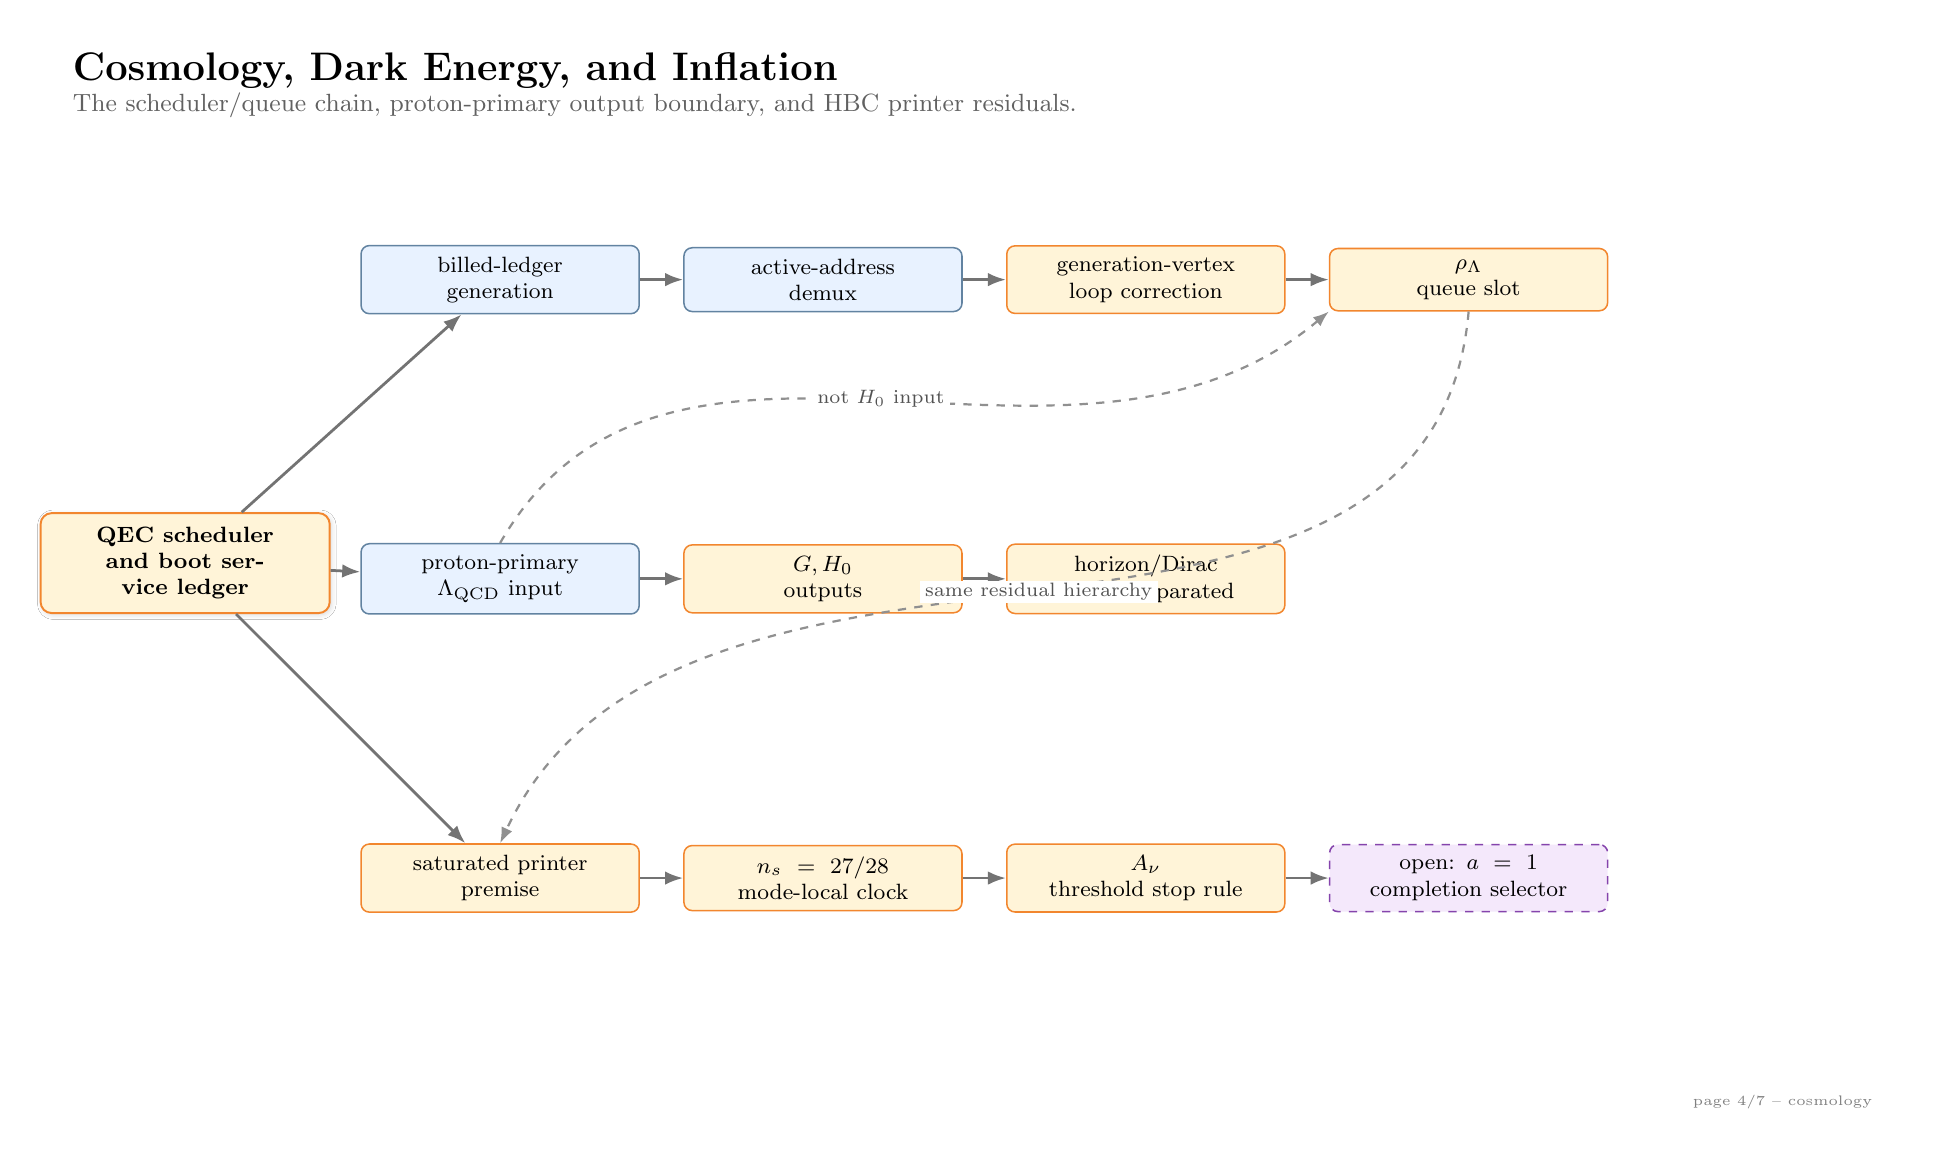
\begin{tikzpicture}[x=1cm,y=1cm]
\treepage{Cosmology, Dark Energy, and Inflation}
  {The scheduler/queue chain, proton-primary output boundary, and HBC printer residuals.}
  {page 4/7 -- cosmology}

\node[root, conditional] (root) at (2.0,7.2) {QEC scheduler\\and boot service ledger};

\node[nodebox, derived] (bill) at (6.0,10.8) {billed-ledger\\generation};
\node[nodebox, derived] (demux) at (10.1,10.8) {active-address\\demux};
\node[nodebox, conditional] (loop) at (14.2,10.8) {generation-vertex\\loop correction};
\node[nodebox, conditional] (cc) at (18.3,10.8) {$\rho_\Lambda$\\queue slot};

\node[nodebox, derived] (proton) at (6.0,7.0) {proton-primary\\$\Lambda_{\rm QCD}$ input};
\node[nodebox, conditional] (h0) at (10.1,7.0) {$G,H_0$\\outputs};
\node[nodebox, conditional] (dirac) at (14.2,7.0) {horizon/Dirac\\history separated};

\node[nodebox, conditional] (sat) at (6.0,3.2) {saturated printer\\premise};
\node[nodebox, conditional] (tilt) at (10.1,3.2) {$n_s=27/28$\\mode-local clock};
\node[nodebox, conditional] (amp) at (14.2,3.2) {$A_\nu$\\threshold stop rule};
\node[nodebox, open] (aone) at (18.3,3.2) {open: $a=1$\\completion selector};

\draw[treeedge] (root) -- (bill);
\draw[treeedge] (bill) -- (demux);
\draw[treeedge] (demux) -- (loop);
\draw[treeedge] (loop) -- (cc);
\draw[treeedge] (root) -- (proton);
\draw[treeedge] (proton) -- (h0);
\draw[treeedge] (h0) -- (dirac);
\draw[treeedge] (root) -- (sat);
\draw[treeedge] (sat) -- (tilt);
\draw[treeedge] (tilt) -- (amp);
\draw[treeedge] (amp) -- (aone);
\draw[crossedge] (cc.south) to[out=-95,in=65] node[edgelabel] {same residual hierarchy} (sat.north);
\draw[crossedge] (proton.north) to[out=60,in=220] node[edgelabel] {not $H_0$ input} (cc.south west);

\end{tikzpicture}

% ---------------------------------------------------------------------------
% Page 5: dark sector.
% ---------------------------------------------------------------------------
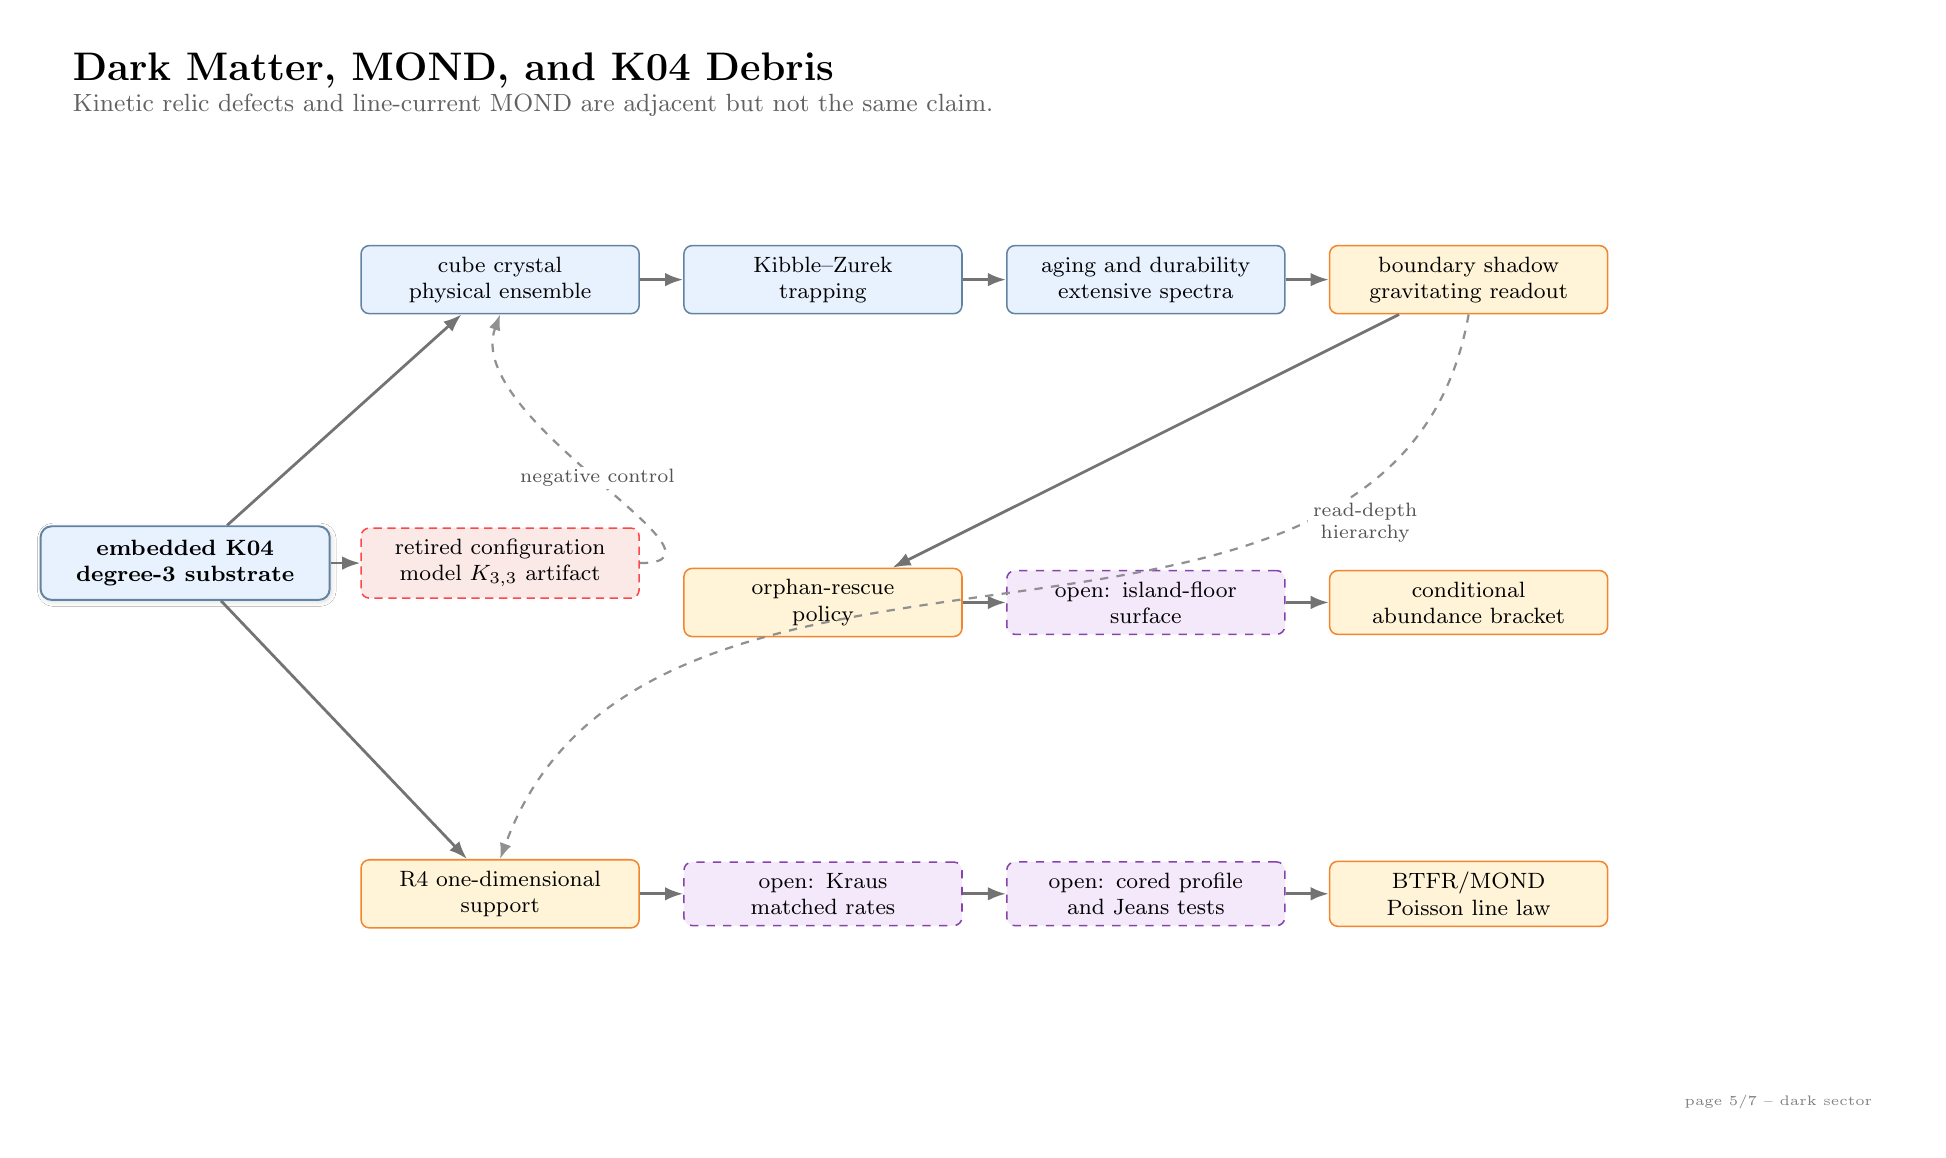
\begin{tikzpicture}[x=1cm,y=1cm]
\treepage{Dark Matter, MOND, and K04 Debris}
  {Kinetic relic defects and line-current MOND are adjacent but not the same claim.}
  {page 5/7 -- dark sector}

\node[root, derived] (root) at (2.0,7.2) {embedded K04\\degree-3 substrate};

\node[nodebox, derived] (cube) at (6.0,10.8) {cube crystal\\physical ensemble};
\node[nodebox, retired] (toy) at (6.0,7.2) {retired configuration\\model $K_{3,3}$ artifact};
\node[nodebox, derived] (kz) at (10.1,10.8) {Kibble--Zurek\\trapping};
\node[nodebox, derived] (dur) at (14.2,10.8) {aging and durability\\extensive spectra};
\node[nodebox, conditional] (shadow) at (18.3,10.8) {boundary shadow\\gravitating readout};

\node[nodebox, conditional] (policy) at (10.1,6.7) {orphan-rescue\\policy};
\node[nodebox, open] (island) at (14.2,6.7) {open: island-floor\\surface};
\node[nodebox, conditional] (abund) at (18.3,6.7) {conditional\\abundance bracket};

\node[nodebox, conditional] (r4) at (6.0,3.0) {R4 one-dimensional\\support};
\node[nodebox, open] (kraus) at (10.1,3.0) {open: Kraus\\matched rates};
\node[nodebox, open] (jeans) at (14.2,3.0) {open: cored profile\\and Jeans tests};
\node[nodebox, conditional] (mond) at (18.3,3.0) {BTFR/MOND\\Poisson line law};

\draw[treeedge] (root) -- (cube);
\draw[treeedge] (root) -- (toy);
\draw[treeedge] (cube) -- (kz);
\draw[treeedge] (kz) -- (dur);
\draw[treeedge] (dur) -- (shadow);
\draw[treeedge] (shadow) -- (policy);
\draw[treeedge] (policy) -- (island);
\draw[treeedge] (island) -- (abund);
\draw[treeedge] (root) -- (r4);
\draw[treeedge] (r4) -- (kraus);
\draw[treeedge] (kraus) -- (jeans);
\draw[treeedge] (jeans) -- (mond);
\draw[crossedge] (shadow.south) to[out=-100,in=70] node[edgelabel, near start, right] {read-depth\\hierarchy} (r4.north);
\draw[crossedge] (toy.east) to[out=0,in=-110] node[edgelabel] {negative control} (cube.south);

\end{tikzpicture}

% ---------------------------------------------------------------------------
% Page 6: gravity and black holes.
% ---------------------------------------------------------------------------
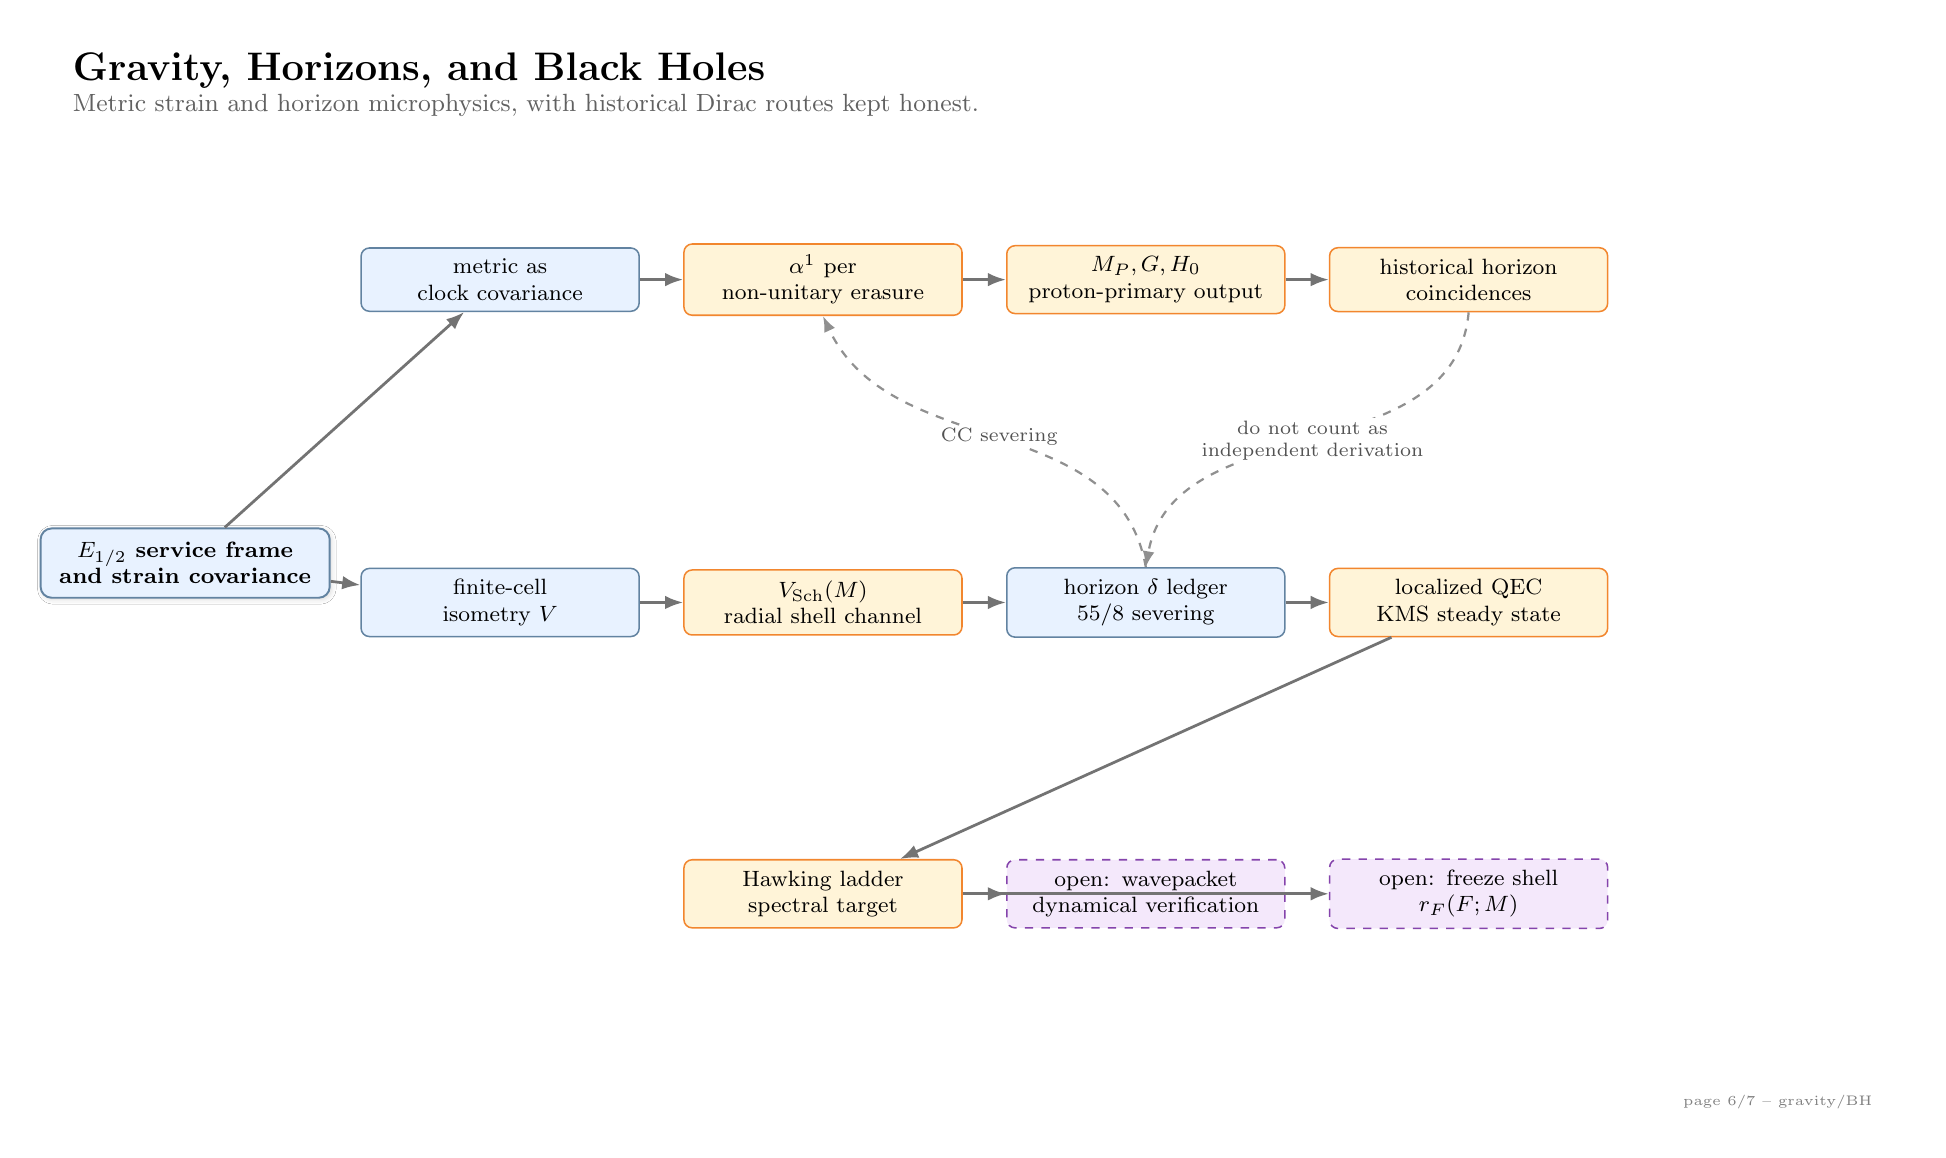
\begin{tikzpicture}[x=1cm,y=1cm]
\treepage{Gravity, Horizons, and Black Holes}
  {Metric strain and horizon microphysics, with historical Dirac routes kept honest.}
  {page 6/7 -- gravity/BH}

\node[root, derived] (root) at (2.0,7.2) {$E_{1/2}$ service frame\\and strain covariance};

\node[nodebox, derived] (metric) at (6.0,10.8) {metric as\\clock covariance};
\node[nodebox, conditional] (alpha) at (10.1,10.8) {$\alpha^1$ per\\non-unitary erasure};
\node[nodebox, conditional] (g) at (14.2,10.8) {$M_P,G,H_0$\\proton-primary output};
\node[nodebox, conditional] (dirac) at (18.3,10.8) {historical horizon\\coincidences};

\node[nodebox, derived] (vcell) at (6.0,6.7) {finite-cell\\isometry $V$};
\node[nodebox, conditional] (vsch) at (10.1,6.7) {$V_{\rm Sch}(M)$\\radial shell channel};
\node[nodebox, derived] (delta) at (14.2,6.7) {horizon $\delta$ ledger\\55/8 severing};
\node[nodebox, conditional] (kms) at (18.3,6.7) {localized QEC\\KMS steady state};

\node[nodebox, conditional] (hawking) at (10.1,3.0) {Hawking ladder\\spectral target};
\node[nodebox, open] (wave) at (14.2,3.0) {open: wavepacket\\dynamical verification};
\node[nodebox, open] (freeze) at (18.3,3.0) {open: freeze shell\\$r_F(F;M)$};

\draw[treeedge] (root) -- (metric);
\draw[treeedge] (metric) -- (alpha);
\draw[treeedge] (alpha) -- (g);
\draw[treeedge] (g) -- (dirac);
\draw[treeedge] (root) -- (vcell);
\draw[treeedge] (vcell) -- (vsch);
\draw[treeedge] (vsch) -- (delta);
\draw[treeedge] (delta) -- (kms);
\draw[treeedge] (kms) -- (hawking);
\draw[treeedge] (hawking) -- (wave);
\draw[treeedge] (hawking) -- (freeze);
\draw[crossedge] (dirac.south) to[out=-95,in=80] node[edgelabel] {do not count as\\independent derivation} (delta.north);
\draw[crossedge] (delta.north) to[out=100,in=-65] node[edgelabel] {CC severing} (alpha.south);

\end{tikzpicture}

% ---------------------------------------------------------------------------
% Page 7: relativity and photon.
% ---------------------------------------------------------------------------
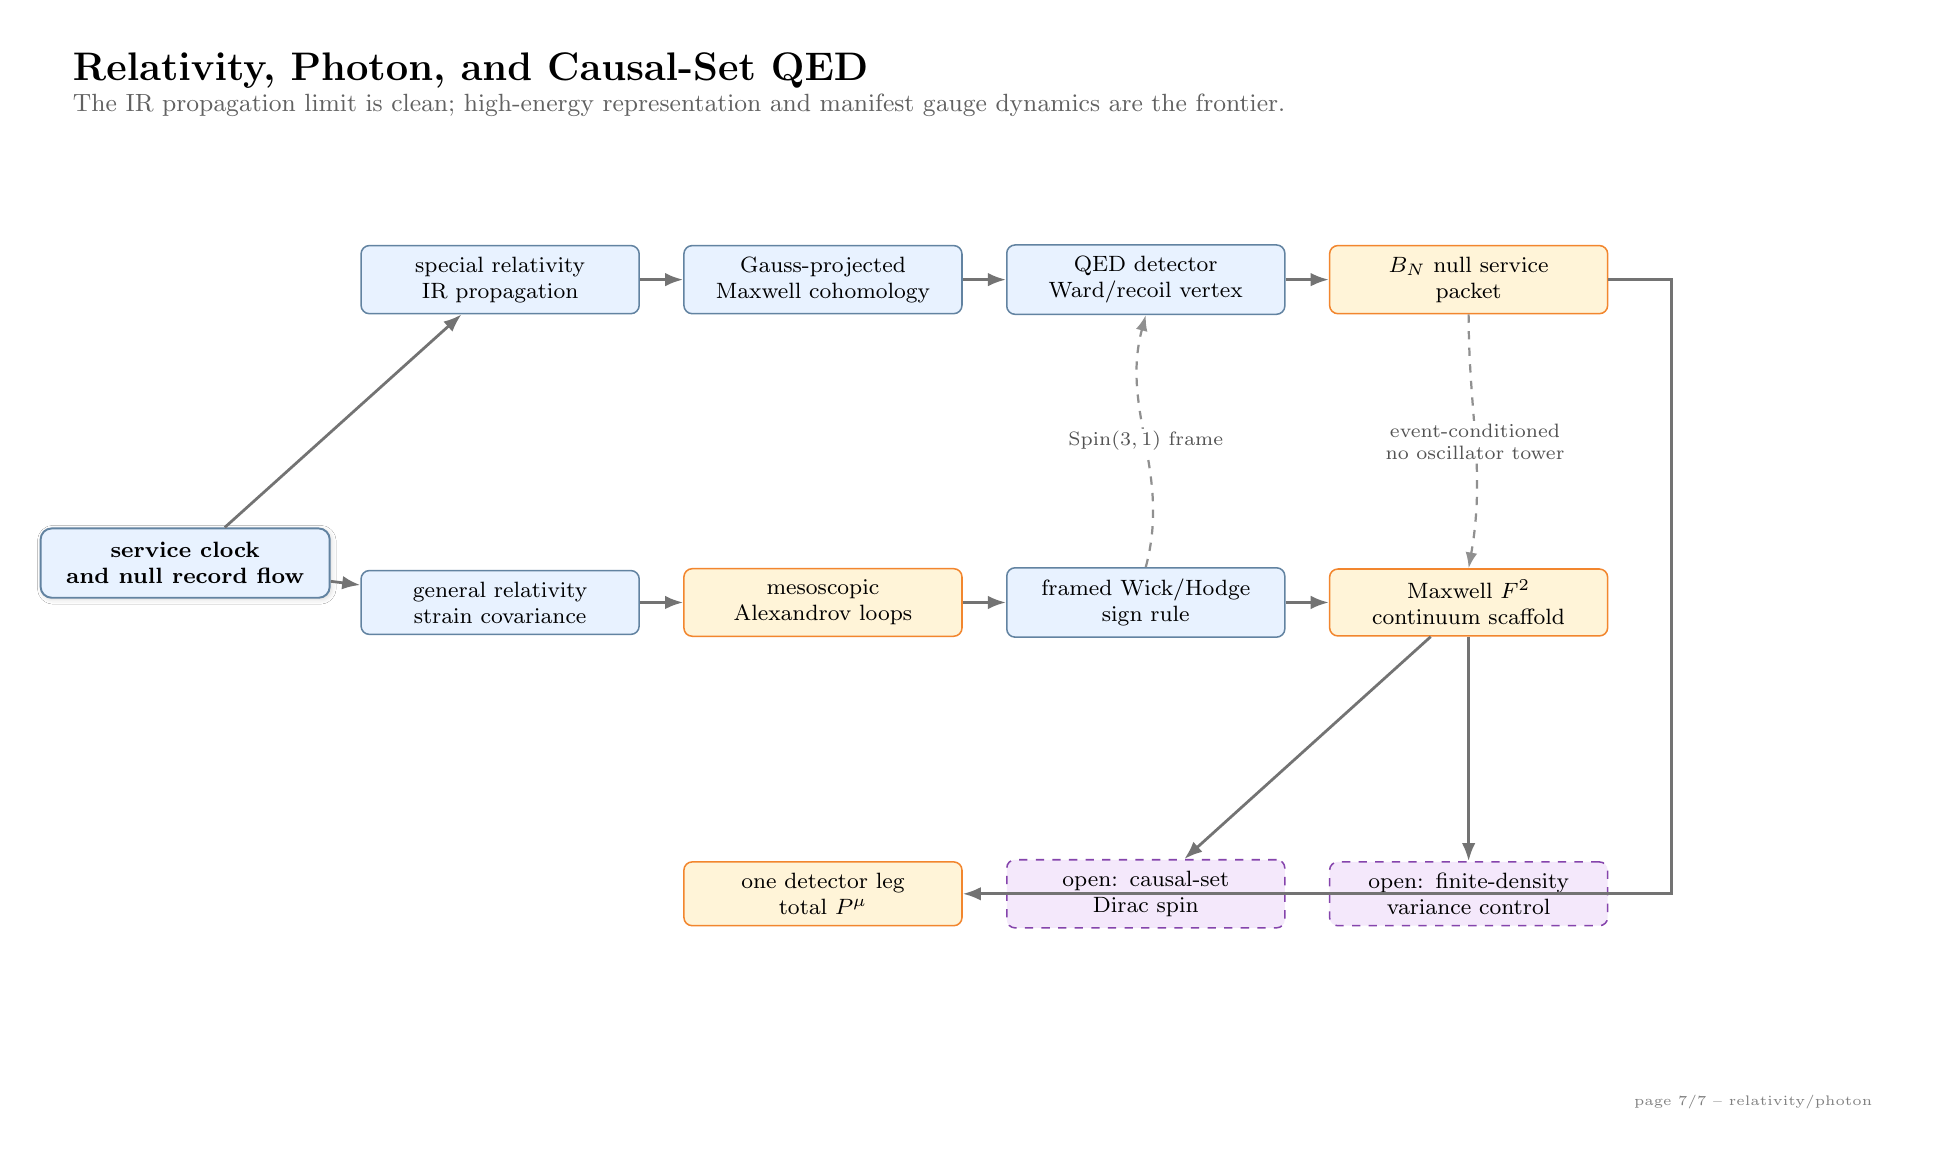
\begin{tikzpicture}[x=1cm,y=1cm]
\treepage{Relativity, Photon, and Causal-Set QED}
  {The IR propagation limit is clean; high-energy representation and manifest gauge dynamics are the frontier.}
  {page 7/7 -- relativity/photon}

\node[root, derived] (root) at (2.0,7.2) {service clock\\and null record flow};

\node[nodebox, derived] (sr) at (6.0,10.8) {special relativity\\IR propagation};
\node[nodebox, derived] (gauss) at (10.1,10.8) {Gauss-projected\\Maxwell cohomology};
\node[nodebox, derived] (ward) at (14.2,10.8) {QED detector\\Ward/recoil vertex};
\node[nodebox, conditional] (bn) at (18.3,10.8) {$B_N$ null service\\packet};

\node[nodebox, derived] (gr) at (6.0,6.7) {general relativity\\strain covariance};
\node[nodebox, conditional] (loops) at (10.1,6.7) {mesoscopic\\Alexandrov loops};
\node[nodebox, derived] (hodge) at (14.2,6.7) {framed Wick/Hodge\\sign rule};
\node[nodebox, conditional] (f2) at (18.3,6.7) {Maxwell $F^2$\\continuum scaffold};

\node[nodebox, conditional] (lsz) at (10.1,3.0) {one detector leg\\total $P^\mu$};
\node[nodebox, open] (spin) at (14.2,3.0) {open: causal-set\\Dirac spin};
\node[nodebox, open] (var) at (18.3,3.0) {open: finite-density\\variance control};

\draw[treeedge] (root) -- (sr);
\draw[treeedge] (sr) -- (gauss);
\draw[treeedge] (gauss) -- (ward);
\draw[treeedge] (ward) -- (bn);
\draw[treeedge] (root) -- (gr);
\draw[treeedge] (gr) -- (loops);
\draw[treeedge] (loops) -- (hodge);
\draw[treeedge] (hodge) -- (f2);
\draw[treeedge] (bn.east) -- ++(0.8,0) |- (lsz.east);
\draw[treeedge] (f2) -- (spin);
\draw[treeedge] (f2) -- (var);
\draw[crossedge] (bn.south) to[out=-90,in=80] node[edgelabel] {event-conditioned\\no oscillator tower} (f2.north);
\draw[crossedge] (hodge.north) to[out=75,in=-105] node[edgelabel] {Spin$(3,1)$ frame} (ward.south);

\end{tikzpicture}

\end{document}
